In order to measure the performance of the locks we measure the time to acquire
$m = 1024$ locks in a row from $n$ number of threads.
Every acquisition loop is repeated 128 times, to ensure that CPU scheduling is not
biasing our data.
Finally, we repeat this procedure for increasing sizes in every lock, for a total
of slightly over 30 million lock acquisitions.

In order to determine these thresholds we ran the algorithm on various sizes and
settled with the first one where no more significant oscillation happened,
in order to remain in the 5 minutes limit imposed on the Nebula back-end.

A further parameter we explored is the size of the critical section.
In all the iterations this is a fixed parameter, where we perform 2, 16, 128,
and 1024 while iterations, to emulate a load that un-trivializes the CS.

Finally, to evaluate the data we collected the time of each acquisition loop in
a CSV with the lock type and size.
We then computed for each lock a $5\%$-trimmed mean\footnote{$\alpha$-trimmed
mean is defined as a compromise between a median and a mean, where we discard
the $\alpha$ portion of the outer values then compute the sample mean on the
remaining ones.}, a robust estimator of the
central tendency.
Due to CPU scheduling in each execution we obtained some outliers that rendered
the data inconsistent.
Using the this robust estimator and collecting a lot of data a very stable
result across runs is ensured: by running the program again, the plots will vary
just slightly, but the main features analysed will persist.

We opted for this measure because it is almost identical to the latency: our
preliminary studies revealed that the behaviour of the $m$ iterations corresponds
to the single lock acquisition time.
This also corresponds to the theory, since the average time to lock is computed
using the sum of the individual lock times, that is the total lock time divided
by $m$.
Therefore, we obtained two plots scaled by a factor $m$.

Furthermore, this measure is the inverse of throughput, therefore sums up the
performance very concisely.

In figure \ref{fig:meantime-2-all} we can observe the performance for all locks,
given CS size 2.
In particular the Filter lock will have a consistently much lower performance
regardless of the CS size, and will be therefore excluded from the following
plots in order to make the data readable.

\begin{figure}[H]
  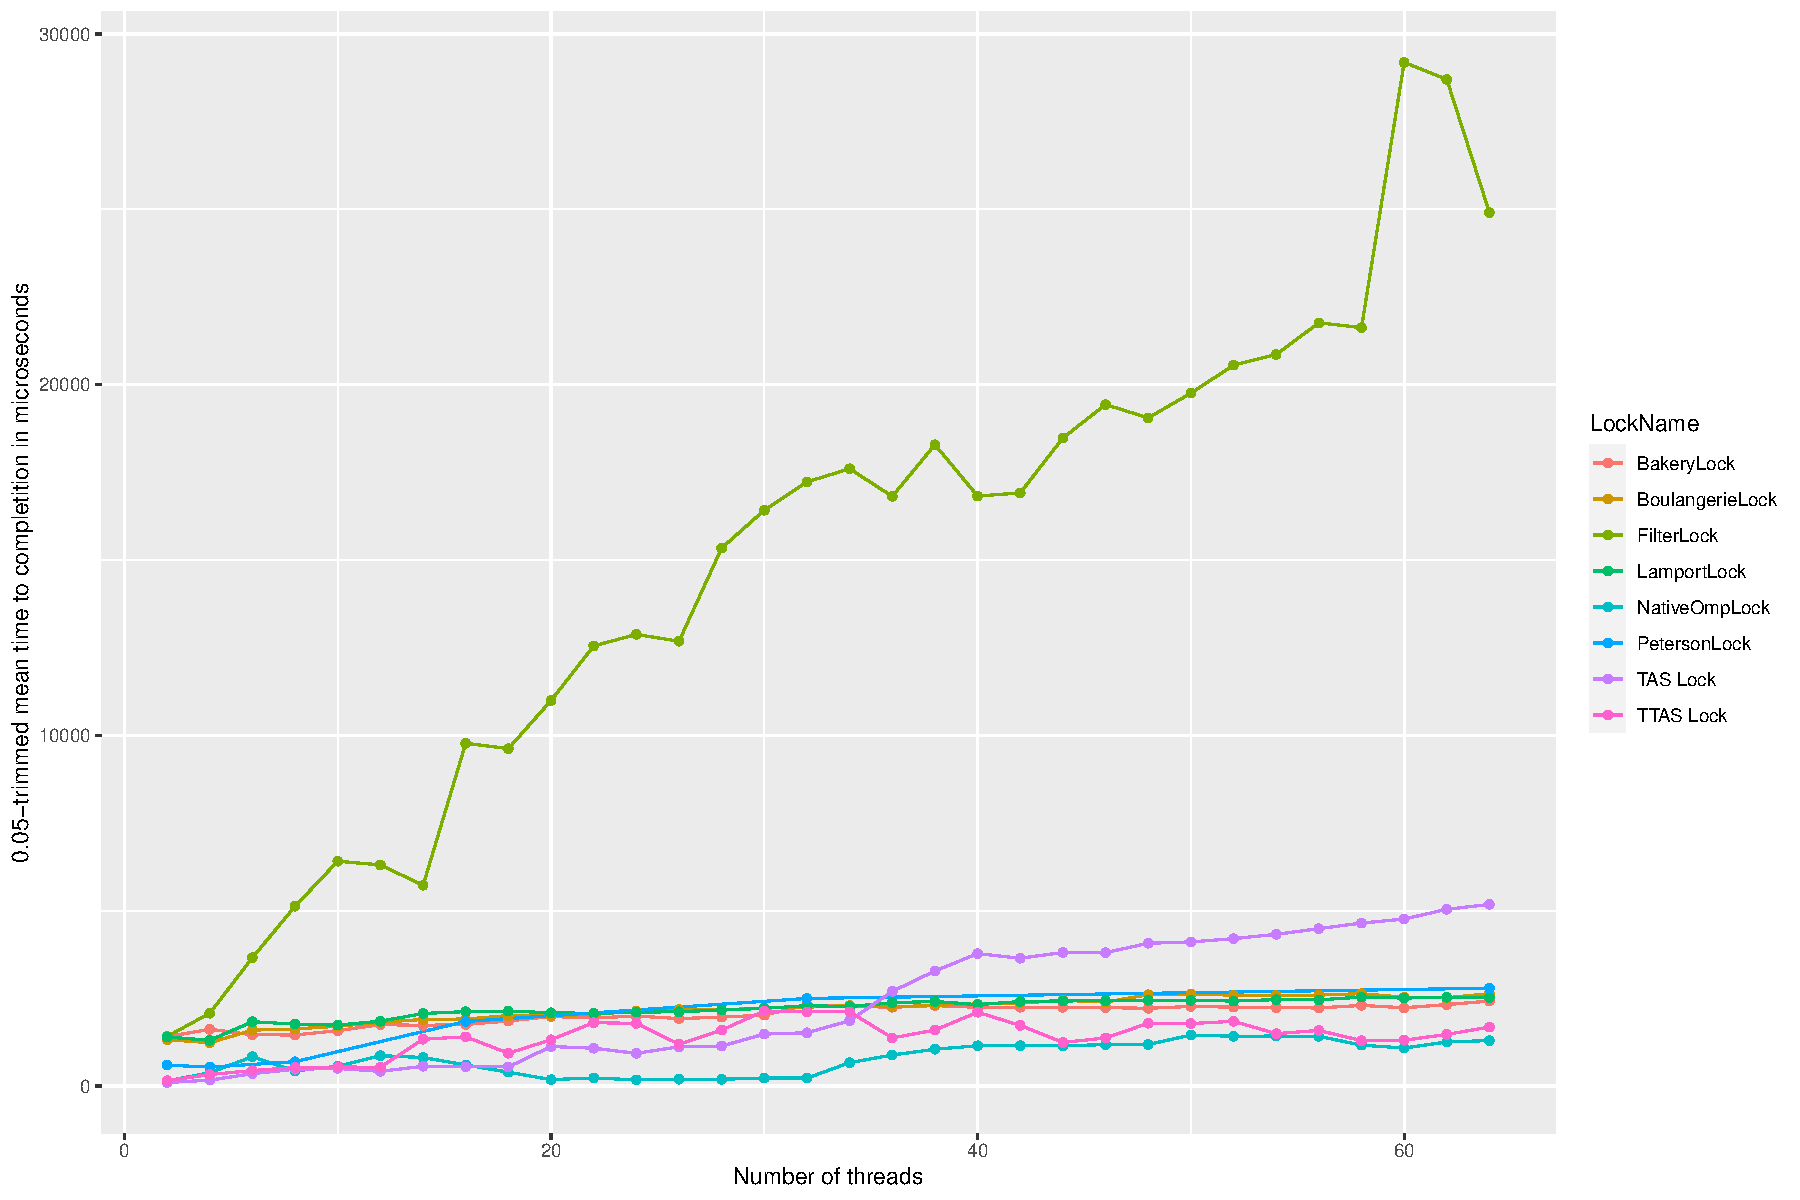
\includegraphics[width=\textwidth]{fig/meantime_2_all}
  \caption{$5\%$-trimmed mean of exec. time of all locks for CS load 2}
  \label{fig:meantime-2-all}
\end{figure}

The other locks, see figure \ref{fig:meantime-2-no-filter} are instead in a similar
range of performance, with the native OpenMP lock and TTAS leading, that maximise
performance at the expense of fairness.
The TAS lock is performant for lower amount of threads, but high contention will
make it the worst lock (except the Filter Lock).
Bakery, Lamport and Boulangerie all behave similarly, with a slow increase in
latency with increasing number of thread, but in a smooth way.
Finally, the Peterson lock offers a very good performance for small locks, i.e.
up to size 8, being also quite fair.
\begin{figure}[H]
  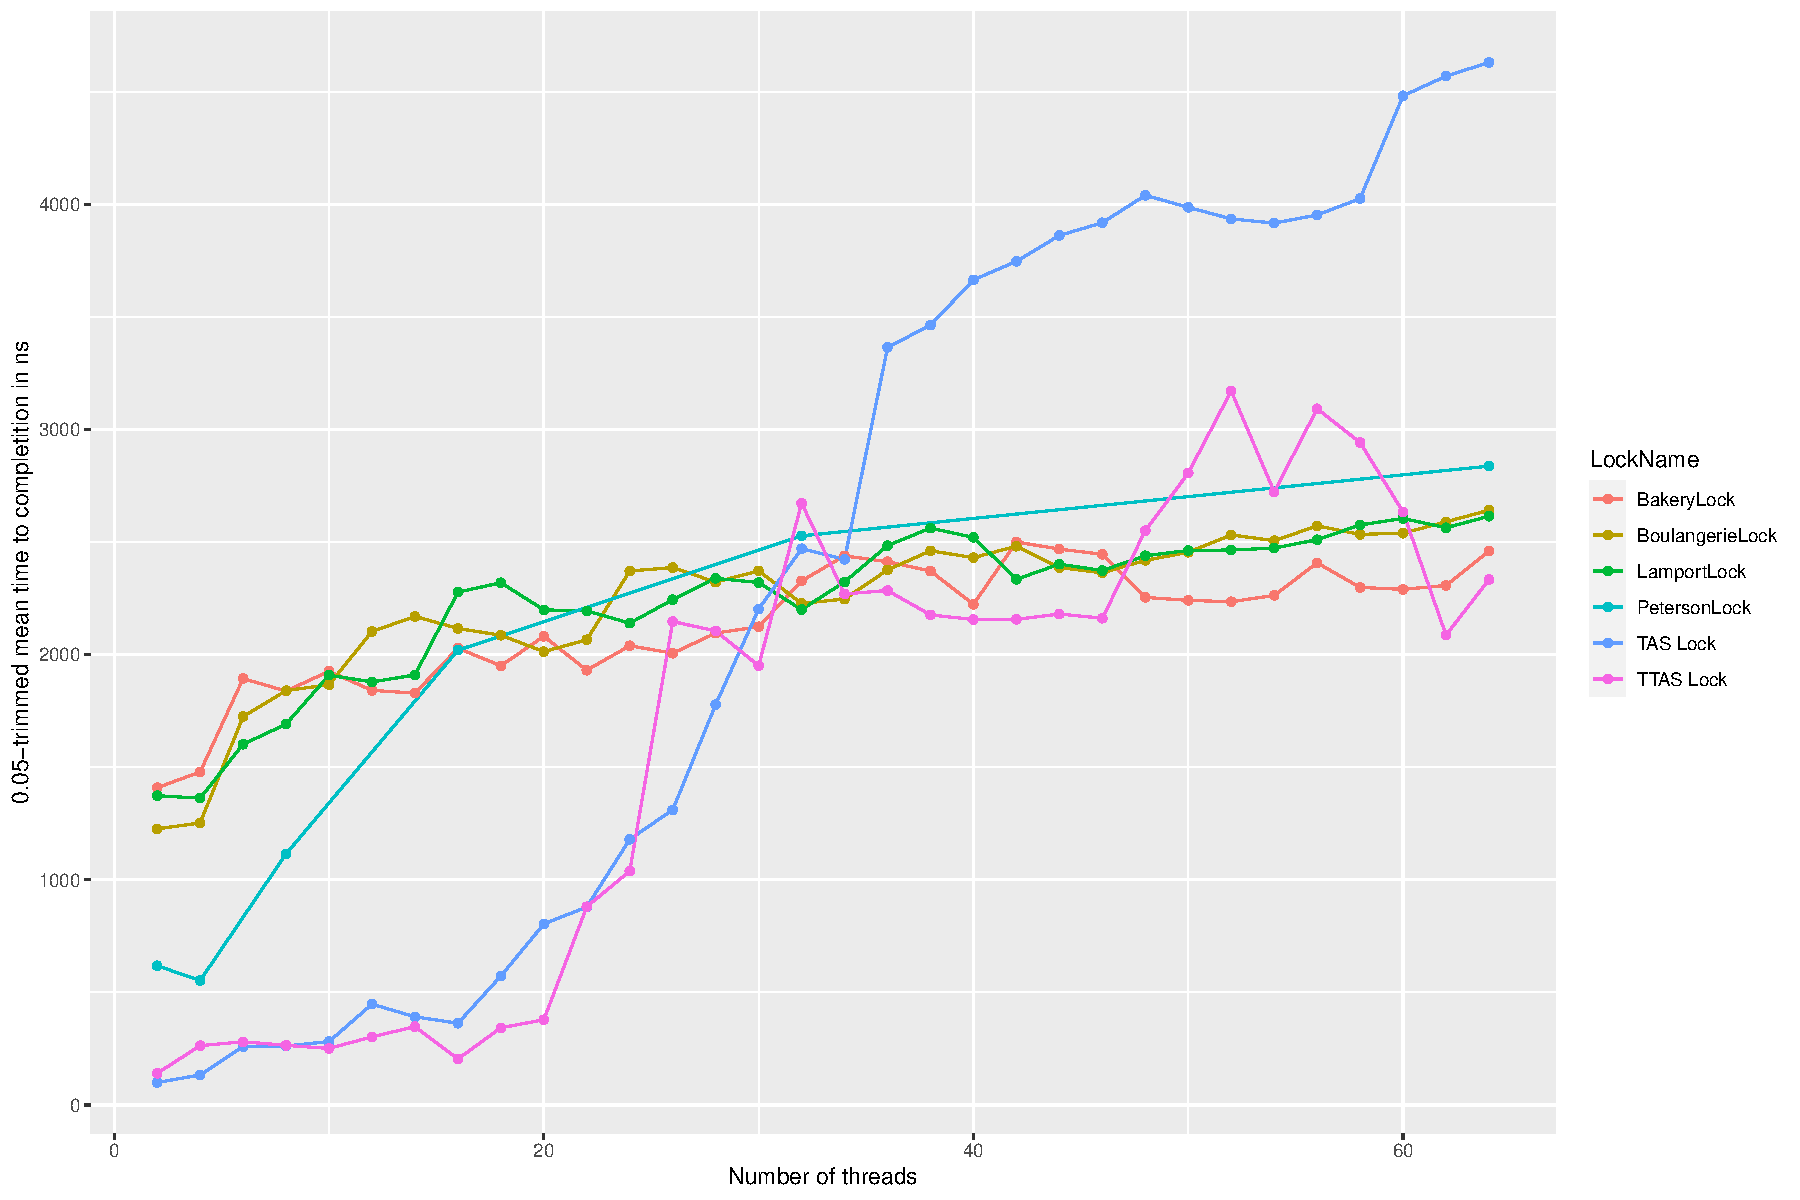
\includegraphics[width=\textwidth]{fig/meantime_2_no_filter}
  \caption{$5\%$-trimmed mean of exec. time of all but Filter lock for CS load 2}
  \label{fig:meantime-2-no-filter}
\end{figure}

We now introduce some load in the CS with parameters with CS size 128 (figure
\ref{fig:meantime-128-no-filter}) and 1024 (figure \ref{fig:meantime-1024-no-filter}).
It is apparent how the TAS lock performs poorly for the high contention
and that the native OpenMP lock consistently performs best, alongside the TTAS.

The Peterson Lock retains its behaviour, with a smooth log-like increase in latency
and the Bakery-based algorithm all perform as a cluster.
It is interesting to notice that the Boulangerie, that should be an improvement
over the Lamport Lock is almost in all cases performing slightly worse.
It can be that on this instruction set (x86\_64) the extra local computation is
actually worsening the algorithm.
The lock was implemented sticking strictly to the paper.

\begin{figure}[H]
  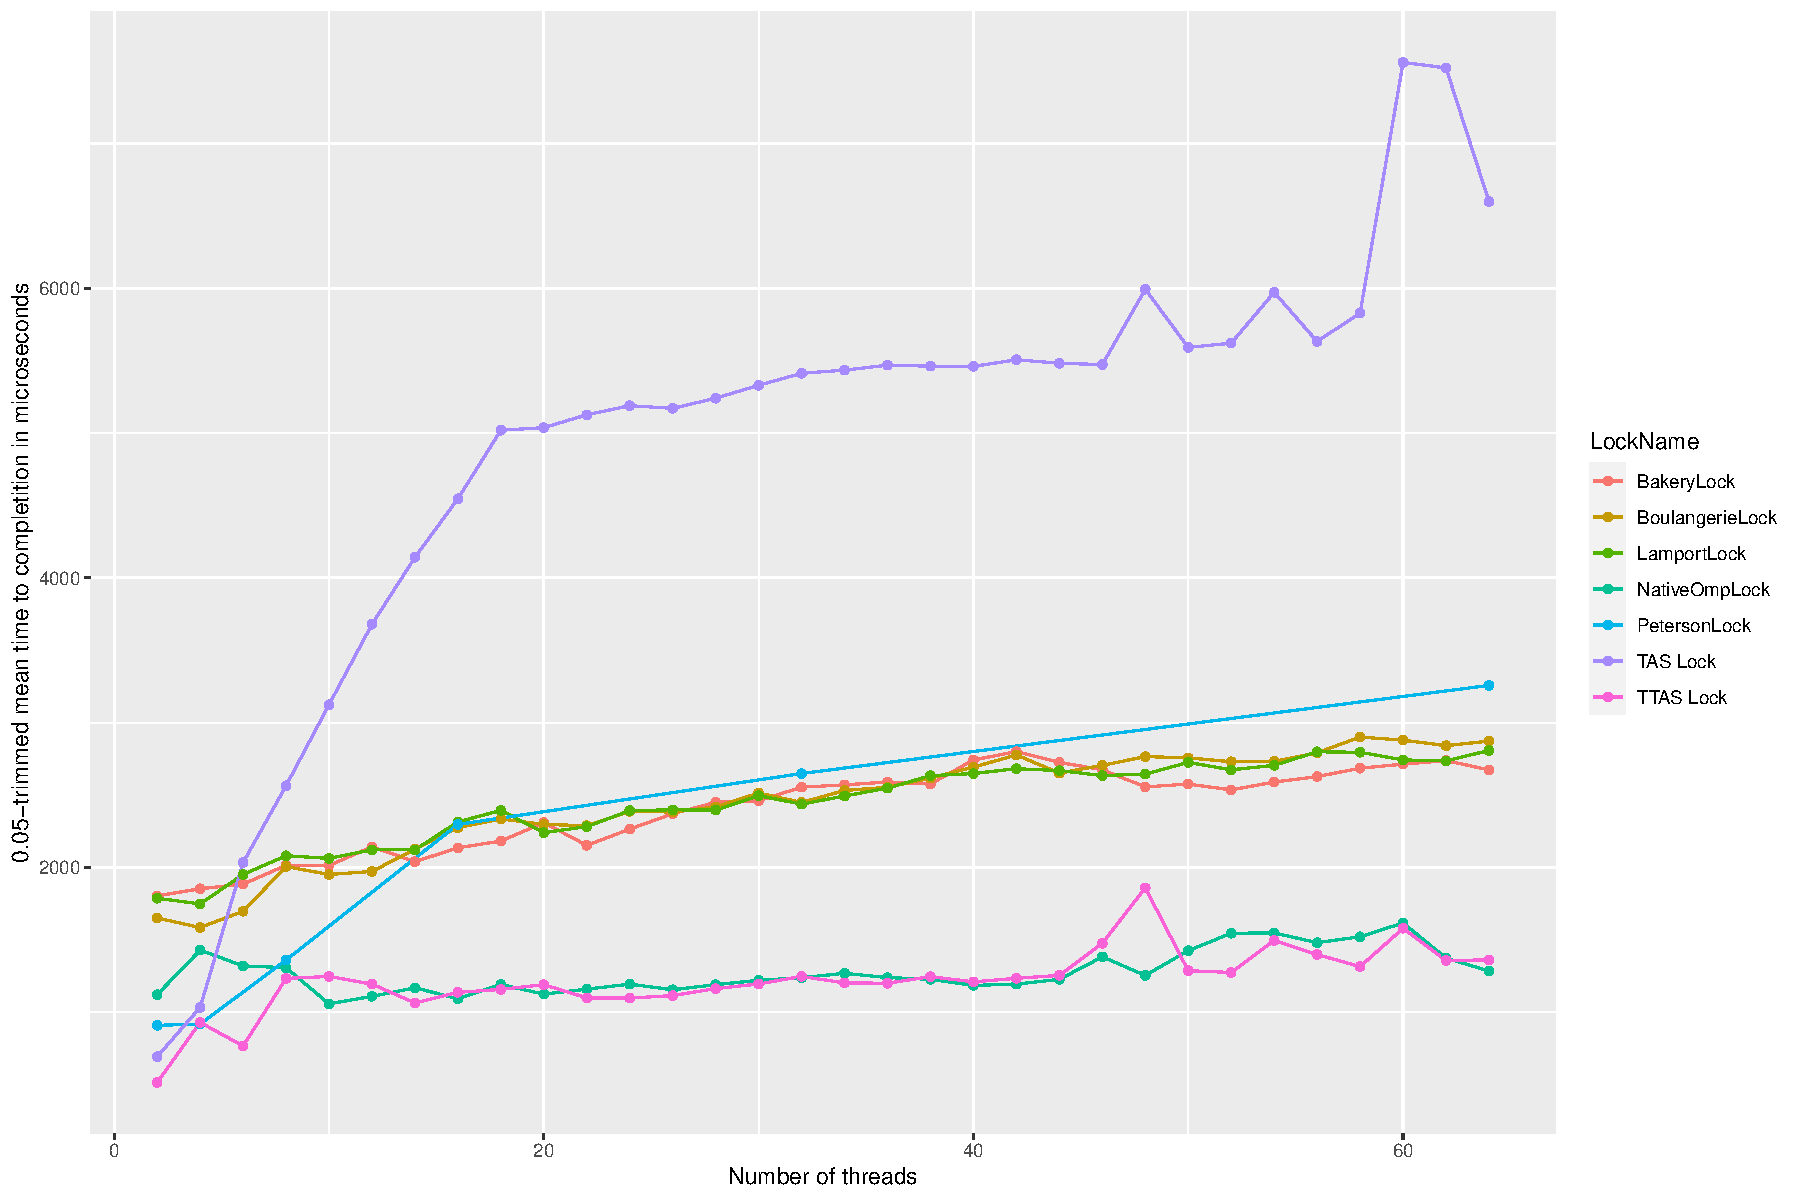
\includegraphics[width=\textwidth]{fig/meantime_128_no_filter}
  \caption{$5\%$-trimmed mean of exec. time of all but Filter lock for CS load 128}
  \label{fig:meantime-128-no-filter}
\end{figure}

\begin{figure}[H]
  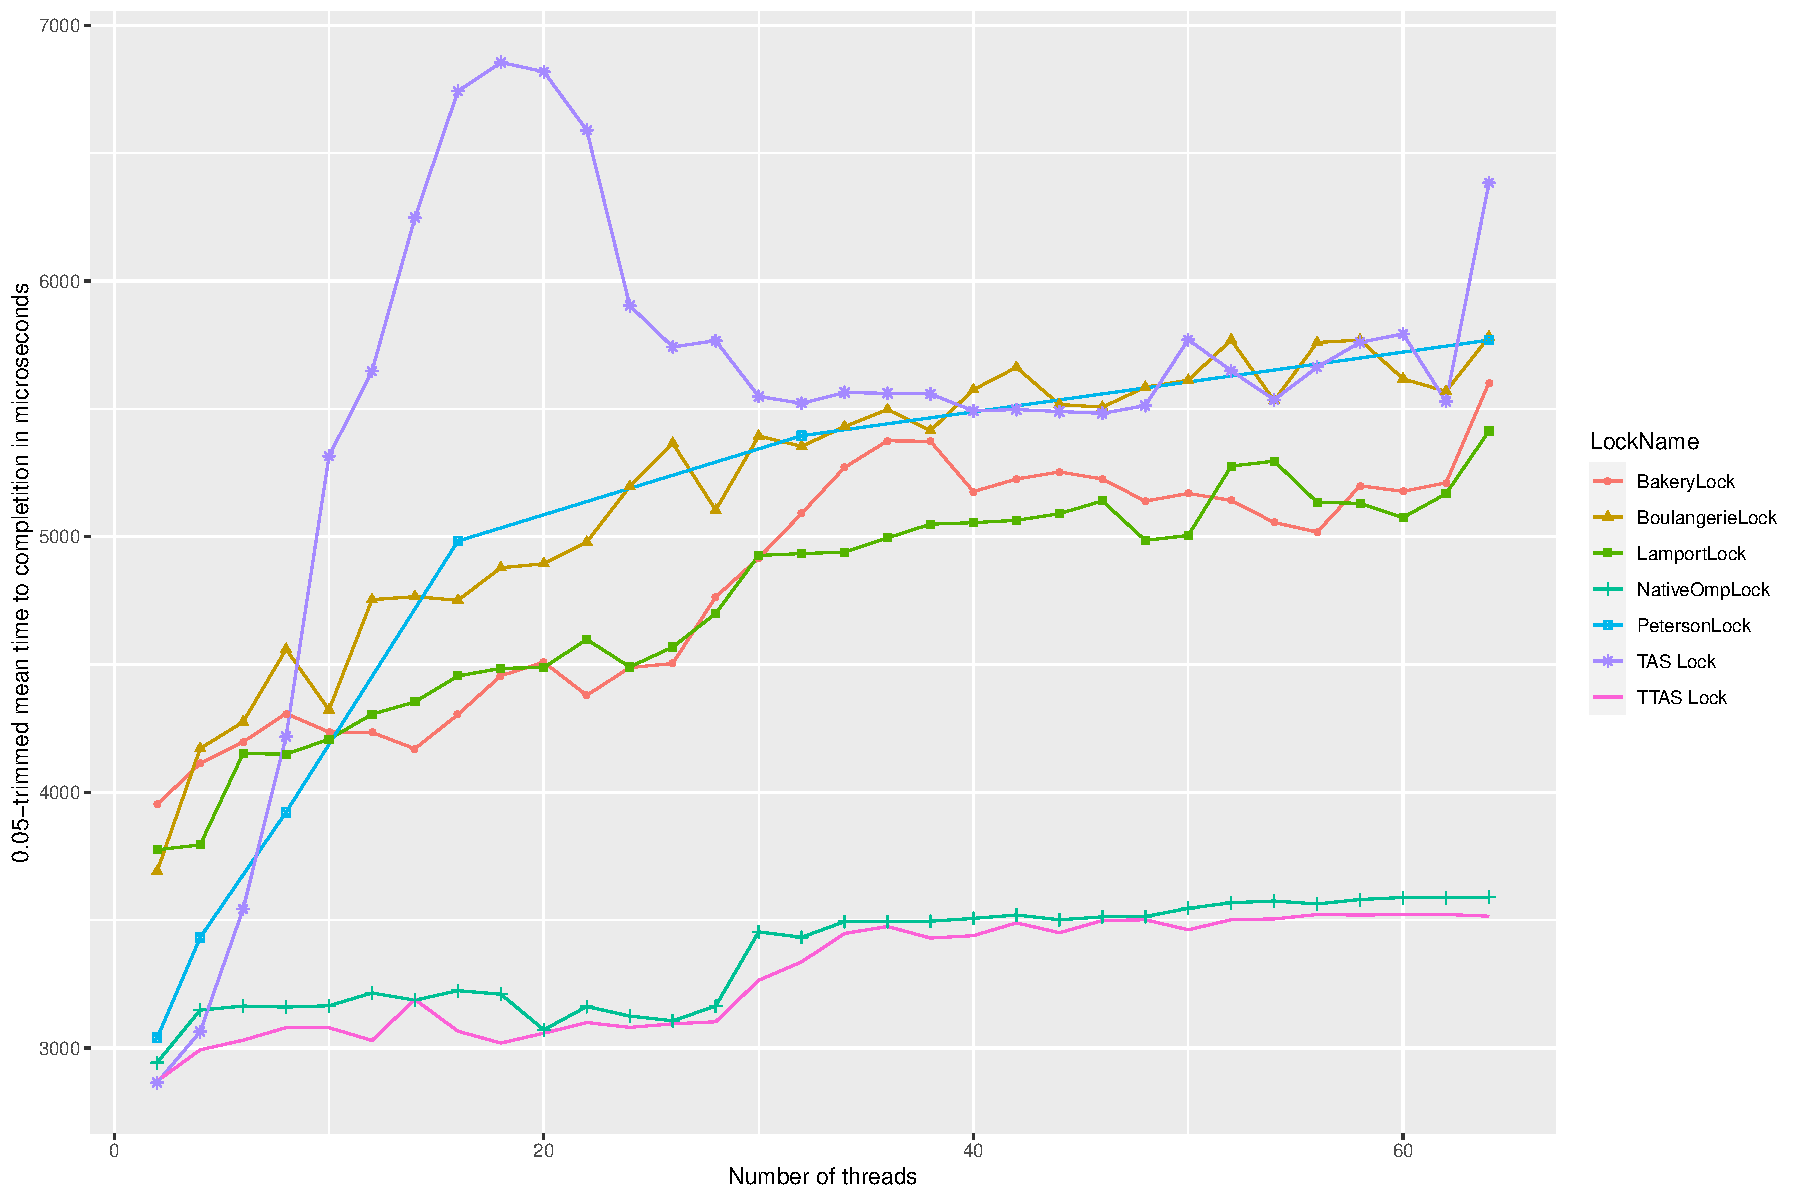
\includegraphics[width=\textwidth]{fig/meantime_1024_no_filter}
  \caption{$5\%$-trimmed mean of exec. time of all but Filter lock for CS load 1024}
  \label{fig:meantime-1024-no-filter}
\end{figure}
